\documentclass[12pt,english]{article}
\usepackage{amsmath}
\usepackage{graphicx}
\graphicspath{{./}}

\title{Temporary Title}
\author{Levi Finkelstein}
\date{\today}

\begin{document}
\maketitle

\section*{Problem 1}

\paragraph{Something here} 
\textit{The problem consists of a few sub-problems that can be partitioned into a group of four identically equations. $\sqrt{7}^2 = 9x^2$ is the first of these.}\\\\
To start we look at this. Which doens't make something like it can't be done.
To start we look at this. Which doens't make something like it can't be done.
\href{https://meme.com}{google}. 
To start we look at this. Which doens't make something like it can't be done.
To start we look at this. Which doens't make something like it can't be done.
2021-08-07

\begin{figure}[h]
    \caption{This is Frank.}
    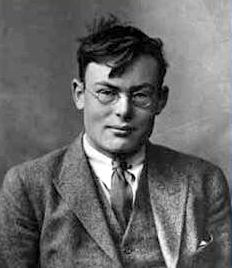
\includegraphics[width=4cm]{frank}
\end{figure}

$$\frac{\partial x}{\partial y} = f(y)$$
$$\begin{pmatrix}
    1&2\\3&4
\end{pmatrix}$$
$$f(x)=\begin{cases}
    a&x>2\\b&x\leq2
\end{cases}$$
$$\lim_{x\to5}f(x)=2$$
The quick brown fox jump
\begin{center}
    \begin{tabular}{cccc}
            & & 3 & 4 \\
            & 1 & 2 & 6 \\
            \hline
        + & 1 & 2 & 6 \\
    \end{tabular}
\end{center}
\newpage

\paragraph{New something}
\textit{ Figure something out.}
$$2+2=\framebox{$4$}$$

\paragraph{Other something}
\textit{ Figure something out.}

$$\frac{1}{2} \Rightarrow 1/2$$
$$\Rightarrow 2\pm2$$

\end{document}
